%!TEX root = ../../main.tex

I dette afsnit beskrives aktører og deres rolle i systemet. I figur \ref{photo:Aktor} ses aktørdiagram, som beskriver alle aktører og deres forhold til systemet

\fixme{Planter skal fjernes som aktør i aktør diagram}

\begin{figure}[H]
	\centering
	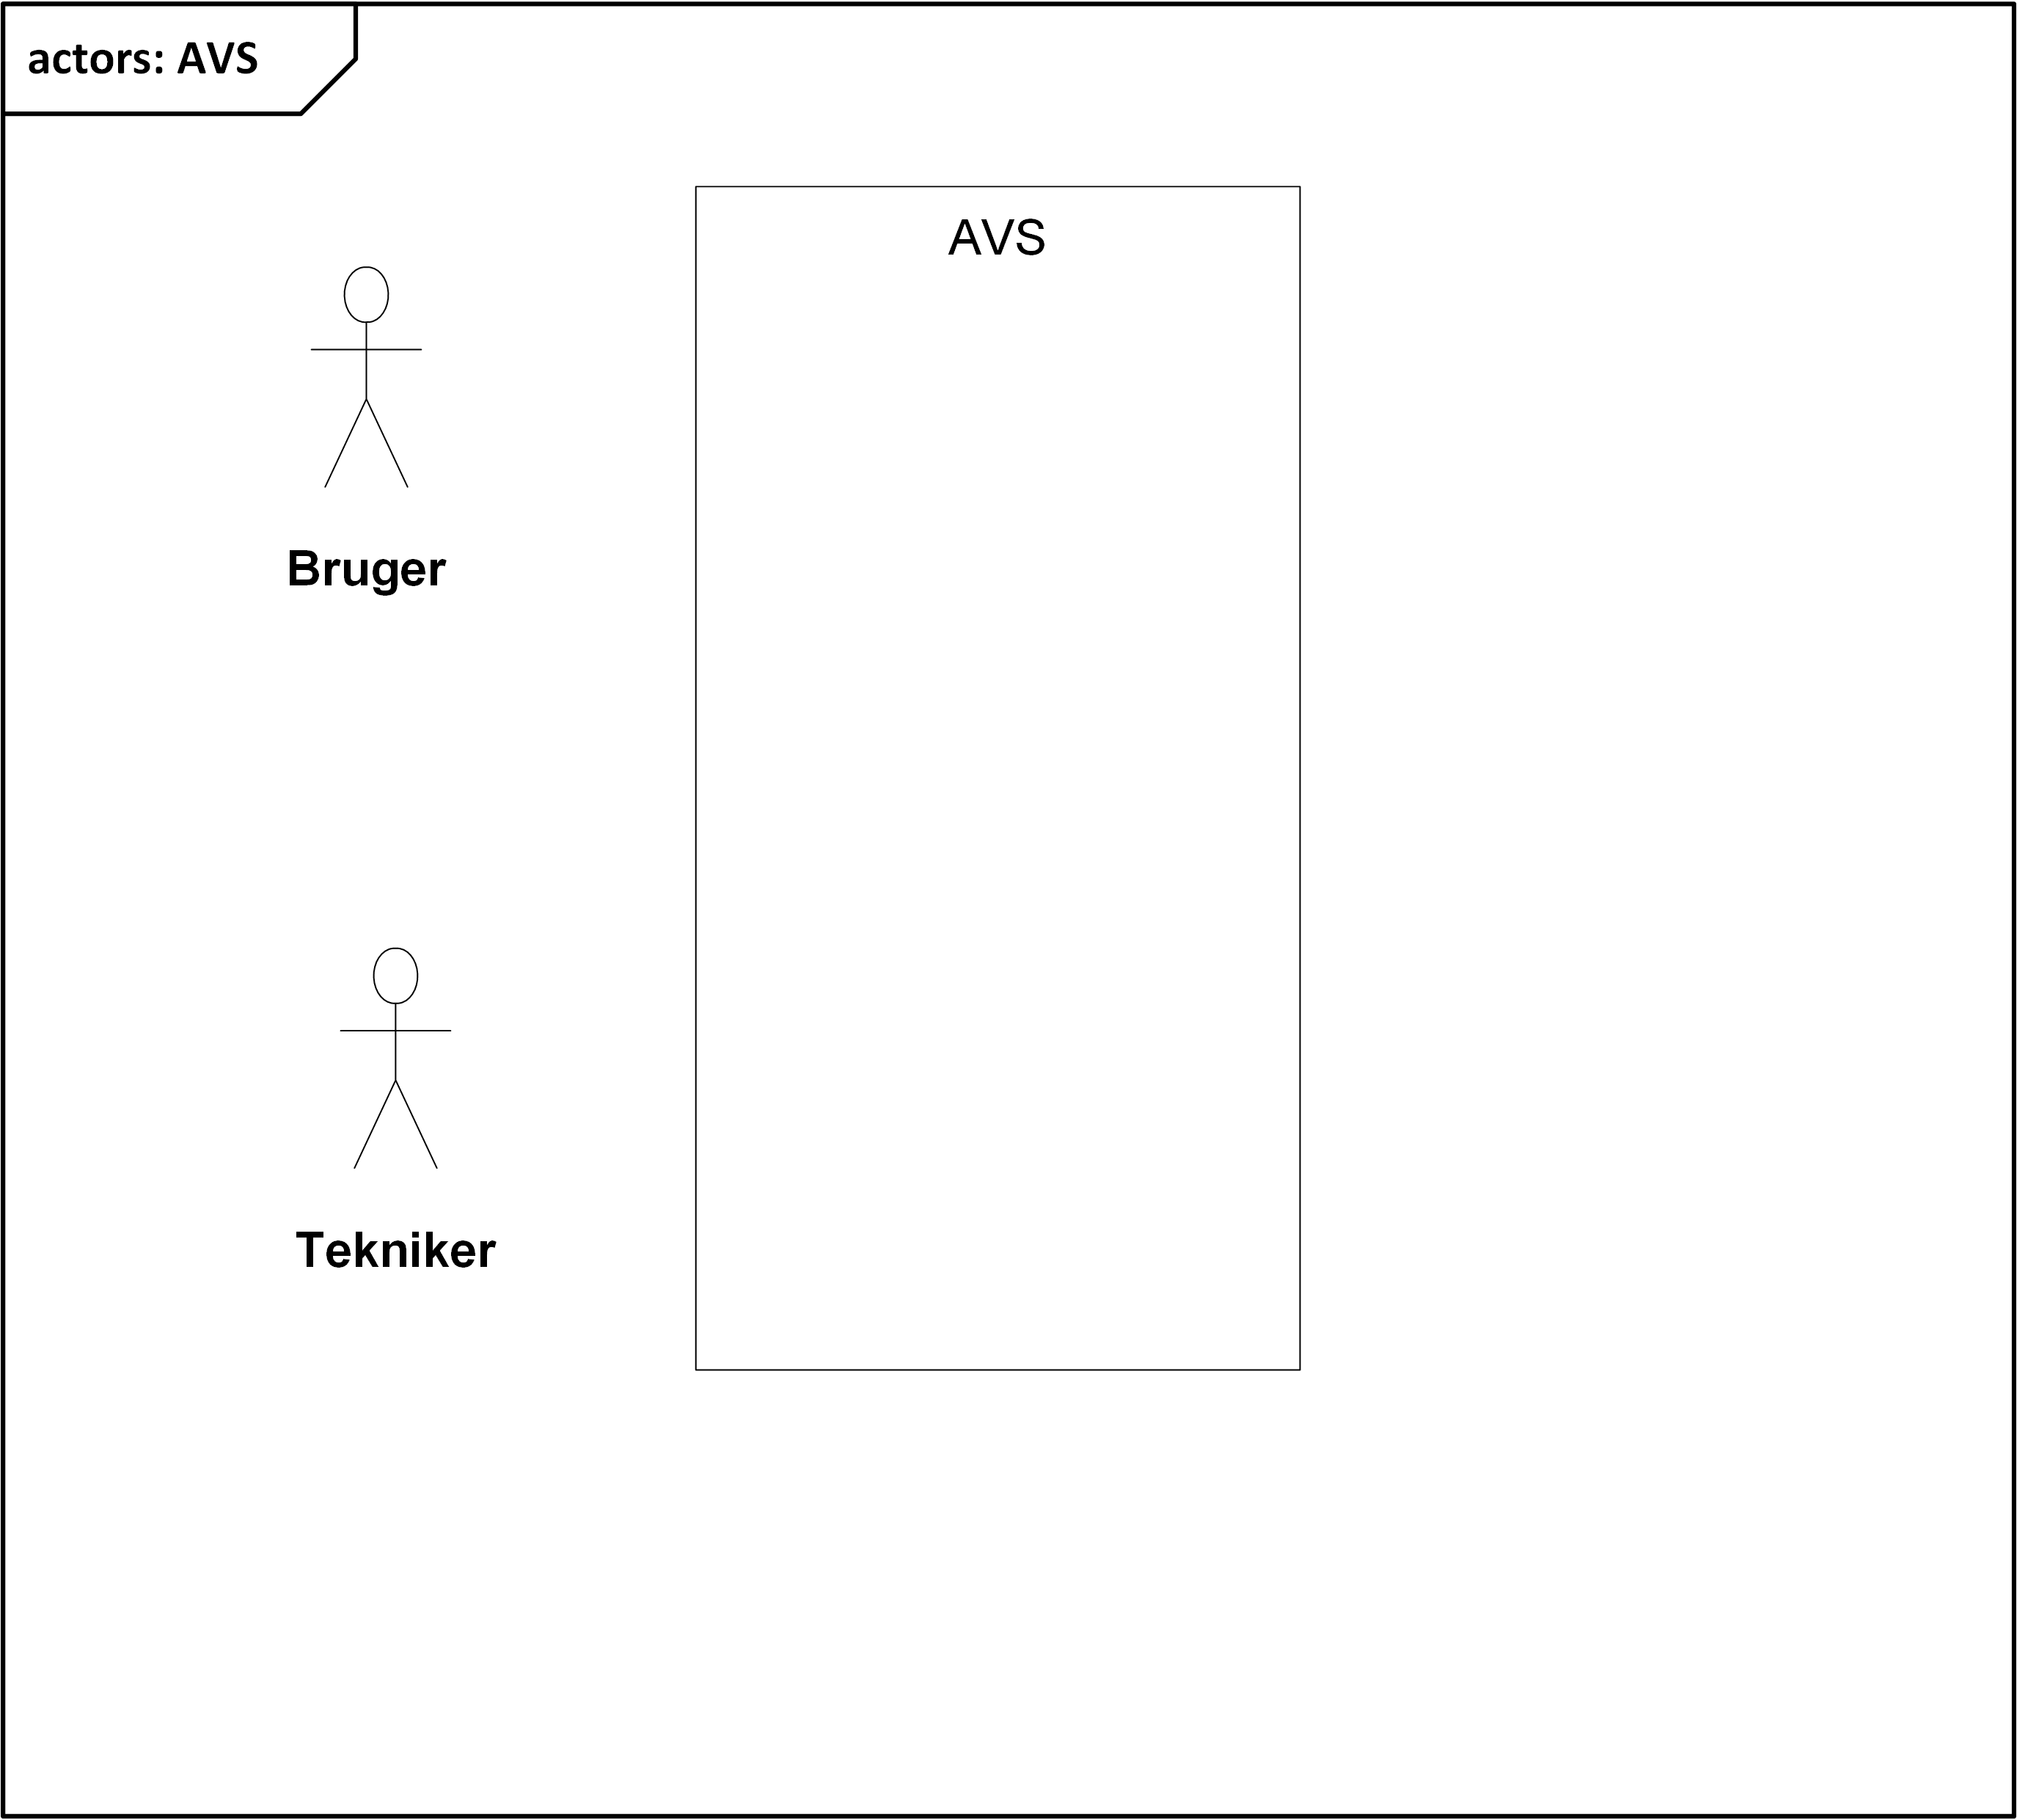
\includegraphics[scale=1]{Kravspecifikation/Actor/Photo/AVS_Actors}
	\caption{AVS Aktører}
	\label{photo:Aktor}
\end{figure}

\fixme{Planter skal fjernes som aktør i aktør beskrivelse}

\subsection{Bruger}
\begin{usecase}
\addtitle{Aktørnavn}{Bruger} 
\addfield{type:}{Primær}
\addfield{Beskrivelse:}{Brugeren er ham, som til dagligt tilgår systemet. Han ved hvor meget gødning og fugtighed planterne skal have, og angiver disse værdier i brugergrænsefladen. Det er brugeren som løbende ændrer værdierne, så systemet hele tiden er opdateret med værdier der passer til planternes vækststadier.}
\end{usecase}

\subsection{Tekniker}
\begin{usecase}
\addtitle{Aktørnavn}{Tekniker} 
\addfield{type:}{Primær}
\addfield{Beskrivelse:}{Teknikeren er en specielt uddannet person. Han har den nødvendige viden om systemet til at kunne installere systemet fra opstart, opsætte nye vandkar mv. En Bruger kan også være tekniker.}
\end{usecase}


\subsection{Planter}
\begin{usecase}
\addtitle{Aktørnavn}{Planter} 
\addfield{type:}{Sekundær}
\addfield{Beskrivelse:}{En plante, som systemet skal kunne vande. Planter består desuden også af et gromedie (jord, lega, mv.), som er det, der reelt bliver vandet.}
\end{usecase}

